\chapter{Produkt Udvikling} \label{chap:ProduktUdvikling}

Ud fra de præsenterede udkast fra undervisningen har vi som gruppe valgt at udvikle et spil med udgangspunkt i en SpaceShip interstellar travel mission. 
På baggrund af de obligatoriske krav og forventninger, har vi analyseret de forskellige muligheder og herefter udvalgt en række minimumskrav, som danner fundamentet for spillets funktionalitet og design. Disse krav sikre at at vores projekt lever op til kursets læringsmål, samtidig med at de giver et godt fundament for videreudvikling af projektet. 
Vi har udvalgt følgende minimumskrav:

\section{Undervisningskrav} \label{chap:ProduktUdvikling_sec:MandatoryRequirement}
\vspace{0.5em}

\begin{itemize}
    \setlength{\itemsep}{5pt}
    \setlength{\parskip}{0pt}
    \setlength{\parsep}{0pt}
    \item Asteroids/planets with potential field effect (gravity, electric, magnetic, black hole or other)
    \item Game levels with increasing speed controlled by the timer/IRQ
    \item 3+ stages docked spaceship
    \item 3+ bullet types with 5+ shot angles
    \item Power-ups
    \item Number of lives on LCD and PC, number of points on LCD and PC, score / high score on LCD and PC
    \item Menu, help screen, and boss key
    \item Multiple bullets
    \item Random delta-angle
    \item Score / High score
    \item Show info on RGB LED
    \item Game controlled by 30010 joystick
    \item Partial/full game on the LCD
\end{itemize}

Med udgangspunkt i kursets obligatoriske krav herover samt den overordnede retning som vi ønsker at trække spillet hen imod, har vi lagt grundlaget for spillets funktionalitet og design. I denne proces har vi taget højde får både de tekniske rammer, der er sat af, den anvendt hardware, samt de læringsmål som projektet har til formå at opfylde.
I følgende afsnit uddybes først de yderligere kravspecifikationer, som vi selv har defineret på baggrund af den idé vi har visualiseret \ref{chap:ProduktUdvikling_sec:VoresKrav}.
Herefter præsenteres spillets overordnede formål og opbygning \ref{chap:ProduktUdvikling_sec:VoresSpil}. 

\vspace{10em}

\section{Kravspecifikationer og implementering} \label{chap:ProduktUdvikling_sec:VoresKrav}
\vspace{0.5em}

For at sikre, at ovenstående krav realiseres i praksis, har vi defineret konkrete kravspecifikationer og tilhørende implementeringsmetoder:

\textbf{Stigende hastighed over tid}
\\Spillets sværhedsgrad øges gradvist ved, at den overordnede spil-hastighed forøges mellem faste tidsintervaller. Dette er implementeret ved hjælp af en timer, som efter hvert interval øger bevægelseshastigheden spillets elementer, hvilket skaber en naturlig stigning i sværhedsgraden.

\textbf{Ændring af spillerens størrelse (Docked spaceship)}
\\Spillerens figur ændres gradvist størrelse i takt med spillets progression. Dette medfører også en stigende sværhedsgrad, da spilleren får mindre manøvrerum. 

\textbf{Power-ups}
\\Der er implementeret flere typer power-ups, som midlertidigt ændrer spillets dynamik. Power-ups vises tilfældigt i spillet og aktiveres ved kollision med spilleren.
\vspace{-0.5em}
\begin{itemize}
    \setlength{\itemsep}{0pt}
    \setlength{\parskip}{1pt}
    \setlength{\parsep}{0pt}
    \item Heart powerup: giver spilleren et ekstra liv
    \item Forcefield powerup: giver spilleren imunitet for projektilerne i 10 sekunder
    \item Multiplier powerup: spilleren vil optjene 2x point de følgende 10 sekunder
\end{itemize}

\textbf{Projektil typer og randomiseret skudretning}
\\Spillet indeholder flere typer projektiler med forskellig hastighed, størrelse og skade. Projekternes skudretning genereres tilfældigt indenfor et defineret vinkelinterval på 60 grader, hvilket bidrager til variation og uforudsigelighed i gameplayet.
\vspace{-0.5em}
\begin{itemize}
    \setlength{\itemsep}{0pt}
    \setlength{\parskip}{1pt}
    \setlength{\parsep}{0pt}
    \item Regular Bullet: mellem fart, mellem hitbox, tager 1 liv
    \item Cannonball: langsom fart, stor hitbox, tager 2 liv
    \item Bouncing Bullet: mellem fart, mellem hitbox, tager 1 liv, hopper tilbage på skærmens top og bund
\end{itemize}

\textbf{Menu og boss key}
\\Spillet indeholder en startmenu med adgang til hjælpeskærm, mulighed for at afslutte spillet og vigtigst af alt, starte spillet. Derudover er der implementeret en boss-key, som giver spilleren mulighed for at pause eller forlade spillet på ethvert tidspunkt.

\textbf{Visuel feedback via RGB LED}
\\RGB LED’en viser spillerens status, hvilket giver hurtig og intuitiv visuel feedback til brugeren. 
\vspace{-0.5em}
\begin{itemize}
    \setlength{\itemsep}{0pt}
    \setlength{\parskip}{1pt}
    \setlength{\parsep}{0pt}
    \item Rød: flasher 0.5 sec efter man mister et liv
    \item Grøn: tændt, men i hviletilstand
\end{itemize}

\textbf{Input via joystick og knapper}
\\Spilleren styrer figuren ved brug af joysticket på NUCLEO boardet (ved at trykke ned på det). Samme joystick bruges til at manøvre gennem menuen og starte spillet. 30010 joysticket vil blive brugt til at "styre" projektilernes bevægelse.

\textbf{Visning af spilinformation på LCD}
\\Liv, score og highscore opdateres løbende på LCD-displayet og i Putt-terminalen, så spilleren har fuldt overblik over spillets tilstand til enhver tid.

\vspace{5em}

\section{Aim of the game} \label{chap:ProduktUdvikling_sec:VoresSpil}
\vspace{0.5em}

Vores spil er opbygget som en "travel mission", med det formål at udforske en mystisk og fremmed planet ude i rummet. Det er et "endless runner game", hvor spilleren forsøger at nå så langt som muligt.
Spilleren bevæger sig op og ned, ved brug af et joystick. Når joysticket holdes ned, bevæger spillerens figur sig op, og ellers bliver figuren trukket ned af planetens tyngdefelt. 
Under spillet bliver der skudt projektiler (bullets) rundt, som spillerne skal undgå. Hvis spilleren bliver ramt, mister man liv afhængigt af typen af bullet. Når spilleren ikke har flere liv tilbage, afslutter spillet. 
Sværhedsgraden i spillet stiger løbende i forhold til tid, dette vil blive gjort ved at implementere flere bullets på hvert level. Tempoet vil sigt samt størrelsen på spilleren, hvilket vil gøre det svære at manøvrere rundt.
For at hjælpe spilleren på vej er der implementere forskellige typer af powerups som vil kunne blive aktiveret løbende.
Spillet fortsætter i et uendeligt loop, indtil spilleren mister alle sine liv, eller vælger at forlade spillet.

\begin{figure}[h]
    \centering    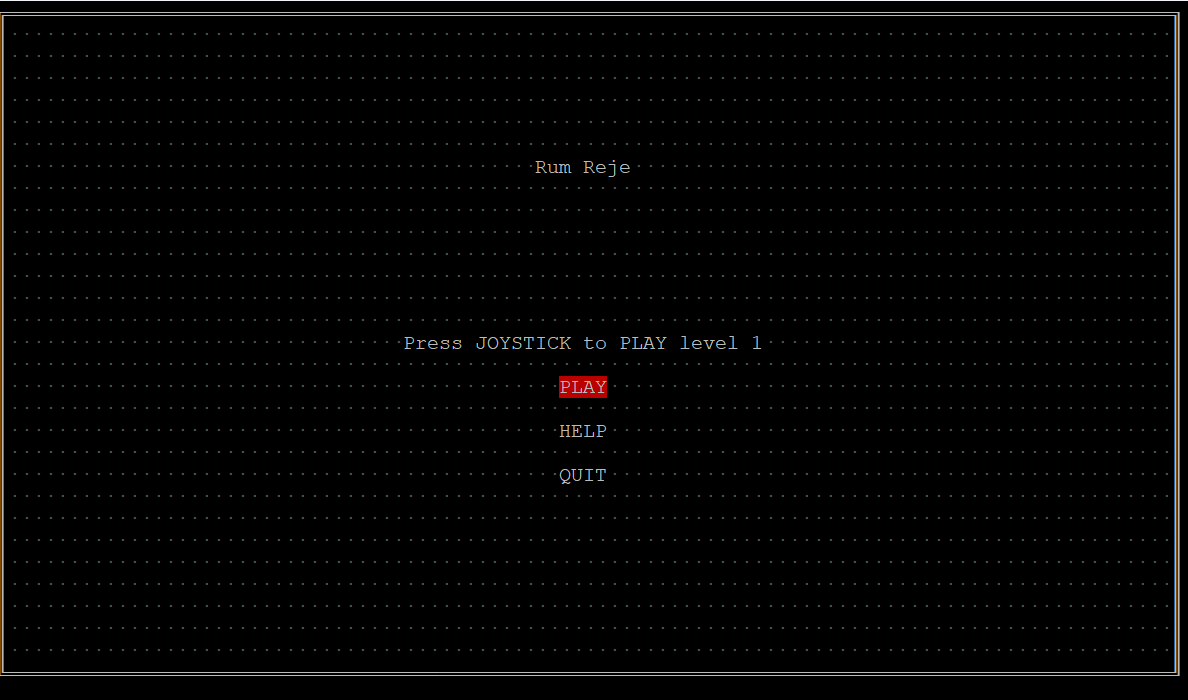
\includegraphics[width=0.74\textwidth]{Picturs/spillet/Screenshot1.png}
    \caption{Billed af spillets "Home screen"}
    \label{fig:spil_billed_1}
\end{figure}
\vspace{-1em}
\begin{figure}[h]
    \centering    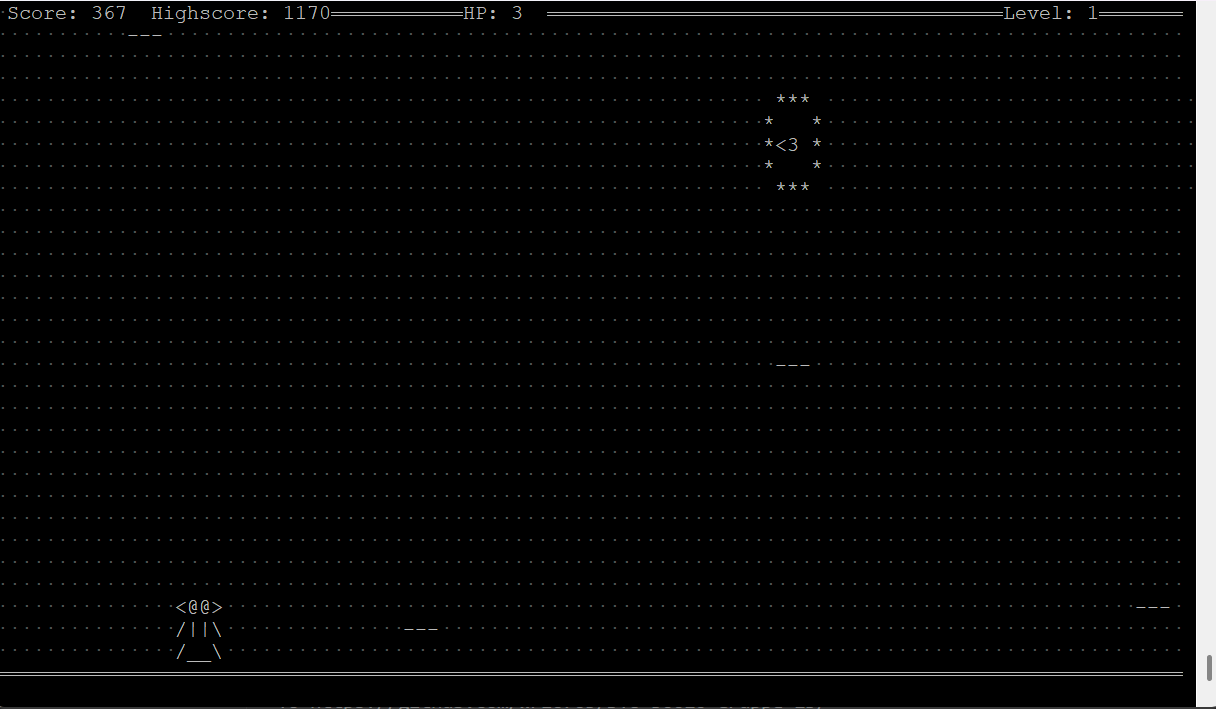
\includegraphics[width=0.74\textwidth]{Picturs/spillet/Screenshot2.png}
    \caption{Billed midt spil}
    \label{fig:spil_billed_2}
\end{figure}
\vspace{-1em}


På figur \ref{fig:spil_billed_1} ses spillets menu. Spilleren kan vælge mellem 3 muligheder. "HELP", som vil føre til en ny side, hvor spilleren kan lærer om reglerne for spillet. "PLAY" som vil starte spillet og "QUIT" som vil forlade spillet.
På figur \ref{fig:spil_billed_2} kan der ses et billede af hvordan spillet ser ud midt-game. Scoren, highscore, liv og level kan ses i toppen af skærmen. Spillerens figur kan ses nede i venstre hjørne og en health powerup kan spottes oppe til venstre. 


\section{Block diagram} \label{chap:ProduktUdvikling_sec:BlockDiagram}
\vspace{0.5em}

For at give et samlet overblik over spillets opbygning og interne struktur er der blevet udarbejdet et blockdiagram. Som illustrerer den overordnede organisering af systemet. Diagrammet repræsenterer projektets overordnet filstruktur og viser samtidigt hvordan spillets funktionalitet er opdelt i separate filer og moduler. Hver block i diagrammet svarer til en central del af koden og afspejler ansvarsfordelingen i projektet.  

\vspace{1em}

\begin{figure}[h]
    \centering    
    
\begin{tikzpicture}[
    box/.style={
        draw,
        rectangle,
        minimum width=3cm,
        minimum height=0.9cm,
        fill=green!30,
        align=center
    },
    arrow/.style={
        -Stealth,
        thick
    },
    node distance=1cm and 0.1cm
]

% Top
\node[box] (main) {main.c};

% Level 2
\node[box, below left =of main] (menu) {menu.c/.h};
\node[box, below right=of main] (gamestate) {games\_state.c};

\draw[arrow] (main) -- (menu);
\draw[arrow] (main) -- (gamestate);

% Level 3
\node[box, below left=of gamestate] (help) {\texttt{helpgameoverpause.c/.h}};
\node[box, below =of gamestate] (physics) {\texttt{Physics.c/.h}};

\draw[arrow] (gamestate) -- (help);
\draw[arrow] (gamestate) -- (physics);

% Level 4
\node[box, below left=of help] (charset) {\texttt{charset.c/.h}};
\node[box, below=of help] (heart) {\texttt{heart.c/.h}};

\node[box, below=of physics] (powerup) {\texttt{powerup.c/.h}};
\node[box, below right=of physics] (bullet) {\texttt{bullet.c/.h}};
\draw[arrow] (help) -- (charset);
\draw[arrow] (help) -- (heart);

\draw[arrow] (physics) -- (powerup);
\draw[arrow] (physics) -- (bullet);
\draw[arrow] (physics) -- (heart);
\draw[arrow] (help) -- (powerup);


% Level 5
\node[box, below=of charset] (adc) {\texttt{adc.c/.h}};
\node[box, below=of heart] (ascii) {\texttt{Ascii.c/.h}};
\node[box, below=of powerup] (gamestateh) {\texttt{game\_state.h}};
\node[box, below=of bullet] (hal) {\texttt{HAL.c/.h}};
\node[box, right=of hal] (io) {\texttt{30010.io}};
\draw[arrow] (charset) -- (adc);
\draw[arrow] (heart) -- (ascii);
\draw[arrow] (powerup) -- (gamestateh);
\draw[arrow] (bullet) -- (hal);
\draw[arrow] (bullet) -- (io);
\draw[arrow] (heart) -- (gamestateh);
\draw[arrow] (heart) -- (adc);
\draw[arrow] (charset) -- (ascii);

\end{tikzpicture}
    \caption{Udkast til block diagram}
    \label{fig:blokdiagram}
\end{figure}

Block diagrammet her over viser den hierarkiske opbygning af projektets filer og den overordnede afhængighed mellem de enkelte moduler. Øverst i diagrammet ses main.c, som fungere som programmets indgangspunkt og koordinere den overordnede afvikling af spillet. Herfra fordeles kontrollen til central styringsmoduler som menu.c og game\_state.c, der håndtere bruger interaktionen samt skiftet mellem spillets forskellige tilstande. 
De under lignende moduler varetager afgrænsede funktioner såsom spilfysik, spilletilstande og positions bestemmelse, mens de nederste moduler hovedsaligt står for input, output og direkte kommunikation med den underliggende hardware. Denne struktur illustrere en klar adskillelse mellem spillets logik og hardwareafhængige funktioner, og danner grundlaget for software arkitekturen, som vi vil komme ind på i næste afsnit.

\vspace{15em}

\section{Software Architecture} \label{chap:ProduktUdvikling_sec:SoftwareArchitecture}
\vspace{0.5em}

Systemet er opdelt i tre lag: et Application Layer, et Application Interface Layer samt et Hardware Abstraction Layer (HAL). Denne lag deling danner grundlaget for en overskuelig opbygning af spillet og sikrer en klar adskillelse mellem spillets regler og den tekniske hardware håndtering.

\begin{figure}[h]
    \centering    
    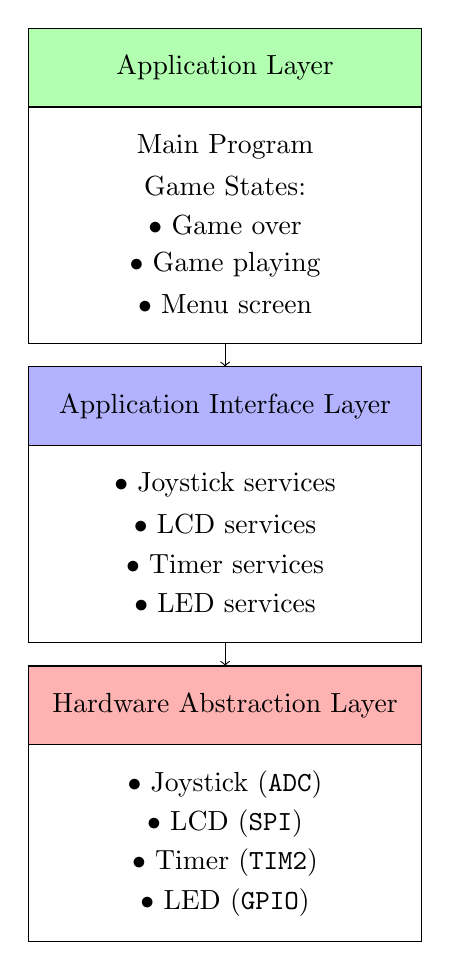
\begin{tikzpicture}
  %first box
  \draw[fill=green!30] (0,0) rectangle (5,-1);
  \draw (0,-1) rectangle (5,-4);
  \draw[->] (2.5,-4) -- (2.5,-4.3);
  %second box
  \draw[fill=blue!30] (0,-4.3) rectangle (5,-5.3);
  \draw (0,-5.3) rectangle (5,-7.8);
  \draw[->] (2.5,-7.8) -- (2.5,-8.1); 
  %third box
  \draw[fill=red!30] (0,-8.1) rectangle (5,-9.1);
  \draw (0,-9.1) rectangle (5,-11.6);


  %titles
  \node at (2.5,-0.5) {Application Layer};
  \node at (2.5,-4.8) {Application Interface Layer};
  \node at (2.5,-8.6) {Hardware Abstraction Layer}; 

  %text in application layer
  \node at (2.5,-1.5) {Main Program};
  \node at (2.5,-2) {Game States:};
  \node at (2.5,-2.5) {$\bullet$ Game over};
  \node at (2.5,-3) {$\bullet$ Game playing};
  \node at (2.5,-3.5) {$\bullet$ Menu screen};
  %text in application interface layer
  \node at (2.5,-5.8) {$\bullet$ Joystick services};
  \node at (2.5,-6.3) {$\bullet$ LCD services};
  \node at (2.5,-6.8) {$\bullet$ Timer services};
  \node at (2.5,-7.3) {$\bullet$ LED services};
  %text in hardware abstraction layer
  \node at (2.5,-9.6) {$\bullet$ Joystick (\texttt{ADC})}; 
  \node at (2.5,-10.1) {$\bullet$ LCD (\texttt{SPI})};
  \node at (2.5,-10.6) {$\bullet$ Timer (\texttt{TIM2})};
  \node at (2.5,-11.1) {$\bullet$ LED (\texttt{GPIO})};  



\end{tikzpicture}
    \caption{Software Architecture diagram}
    \label{fig:Software_arkitektur}
    \vspace{0em}
\end{figure}

\subsection{Application Layer}
Dette lag indeholder spillets overordnede logik og styring. Laget håndterer den overordnede spille logik, samt de forskellige spilde tilstande som, Home Screen, Game Play og Game Over. Laget her er uafhængigt af det underliggende hardware og fokuserer udelukkende på spillets overordnede adfærd og regler.

\textbf{Game Context:} 
Centralt for dette lag er en GameContext struktur (struct), der fungere som spillets hukommelse. Den holder styr på variabler som game\_state, level, score og Highscore.

\textbf{Game State:}
Laget bestemmer hvilket tilstand spilet er i. Altså om systemet skal eksekverer logikken for menuen, selve gameplayet eller hjælpeskærmen. Dette er med til at sikre aspillet reagere korrekt på de logiske overgange.

\textbf{Physics \& Rules:} 
Her beregnes de matematiske regler for spillet, såsom projektil-baner og spillerens bevægelse. Baseret på det data som der bliver leveret fra de underliggende lag. 

\subsection{Application Interface layer}
Laget her fungerer som et bindende lag mellem spillets logik og den underliggende hardware. Det sørger for, at data flyder flydende mellem lagene, men dets primære formål er at gøre koden “portabel”. Dette lag fungerer som "oversætteren" og det afgørende bindeled mellem spillets logik og den specifikke hardware. Ved at isolere de hardware definerede funktioner i dette lag, kan Application Layer i princippet flyttes til en anden platform, uden at spillets kernelogik skal omskrives.

\subsection{Abstraction Layer}
Dette lag indeholder de hardware specifikke funktioner. 
Hardware-delen fokuserer på de moduler, der interagerer direkte med mikrokontrolleren og de eksterne komponenter på 30010-boardet. Dette lag danner fundamentet for systemet ved at transformere fysiske signaler til data så softwaren kan modtage input og give feedback.
Laget sørger for direkte kommunikation med hardwaren og stiller simple funktioner til rådighed for de overliggende lag. 

\textbf{Input-håndtering (Joystick \& Knapper):} 
Som vist i flowchartet afhænger spillets forløb af brugerens input. Her implementeres funktioner til at aflæse de analoge værdier fra joysticket via ADC’en (Analog-to-Digital Converter) samt de digitale input fra knapperne. Disse værdier normaliseres, så spillogikken let kan beregne bevægelse.

\textbf{Visuel Output (LCD \& RGB LED):} 
Denne del af koden styrer opdateringen af LCD-displayet via SPI-kommunikation. RGB LED’en styres her for at give øjeblikkelig feedback på spillerens tilstand, så som tab af liv eller opsamling af power-ups.

\textbf{Timing og Afbrydelser (Timer):} 
For at sikre en stabil spilhastighed benyttes hardware-timere. Dette gør det muligt at opdatere spillets tilstand med en fast frekvens (30 Hz), hvilket er essentielt for en flydende spiloplevelse.

Denne software arkitektur er afgørende for projektets samlede robusthed og skalerbarhed. Ved, konsekvent, at adskille hardware abstraktionerne fra spillets regler, sikres en struktur hvor fejlfinding bliver væsentligt lettere, da problemet kan isoleres til specifikke lag uden at påvirke hele systemet. Det gør det muligt at udvikle spillets individuelle funktioner, samtidig med at det holder koden struktureret og læselig.

\section{Systemets overordnede opbygning} \label{chap:ProduktUdvikling_sec:overordnet opbygning}
\vspace{0.5em}

\subsection{Flow diagram af spillet} \label{chap:ProduktUdvikling_sec:flowchart}

\begin{figure}[H]
    \centering
    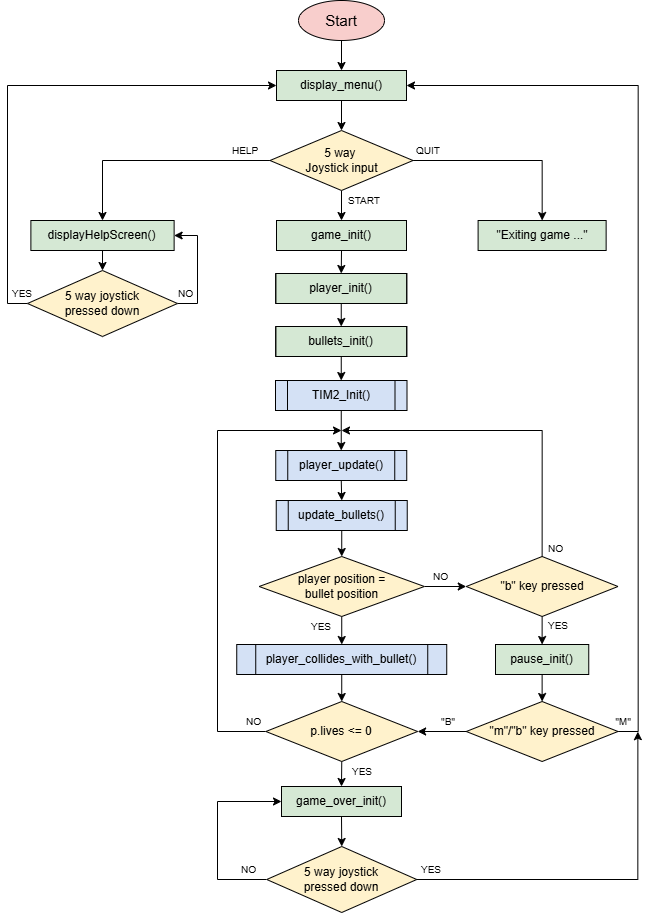
\includegraphics[width=\textwidth]{Picturs/Diagrammer/FINAL_FLOW_FARVER_10000.drawio.png}
    \caption{Flow diagram af vores spil}
    \label{fig:flow_diagram}
\end{figure}

Repræsenteret herover ses et overordnet flowdiagram af vores spil (figur \ref{fig:flow_diagram}). Diagrammet er opbygget efter klassiske flowdiagram-principper, hvor beslutningspunkter anvendes til at håndtere bruger input, og procesbokse beskriver de handlinger og funktioner som systemet udfører. I grøn er initialisering af visuelle output repræsenteret og i blå er spillets fundamentale funktion, som vil blive uddybet følgende (afsnit \ref{chap:ProduktUdvikling_sec:tid&spiller}).

Programmet starter med visning af menuen (\lstinline!display_menu()!), hvor spilleren ved hjælp af et "5-way" joystick kan vælge mellem 3 forskellige muligheder. Afhængigt af det valgte input fortsætter programmet enten til hjælpeskærmen (\lstinline!displayHelpScreen()!), initialisering af spillet (\lstinline!game_init()!) eller afslutning af programmet. 
Når spillet starter initialiseres de nødvendige spilleelementer, herunder spiller (\lstinline!player_init()!) projektiler (\lstinline!bullets_init()!) og timer (\lstinline!TIM2_init()!). Efterfølgende indgår programmet i et opdaterende loop, hvor spillerens og projektilernes tilstand opdateres (\lstinline!player_update()! \& \lstinline!update_bullets()!) og hver der kontinuerligt kontrolleres for kollision mellem disse to (\lstinline!player_collides_with_bullet()!). Under spillet er der mulighed for at pause spillet (\lstinline!pause_init()!) ved hjælp at et tast input. Her har spilleren mulighed mellem at genoptage spillet eller returner til menuen. Spillet fortsætter til alle liv er brugt op, og vil initialisere en game over skærm (\lstinline!game_over_init()!) der vil fremvise spillerens score og highscore, og give spilleren mulighed for at returnere til menuen. 

For at give et mere detaljeret indblik i spillets funktionalitet fokuserer det følgende afsnit på de centrale processer i spillets opdateringsloop. Her uddybes håndteringen af spilleren og projektilernes positioner samt den anvendte kollisionslogik, da disse funktioner er afgørende for spillets interaktion og dynamik.

\vspace{0.5em}
\subsection{level system \& spillerens position} \label{chap:ProduktUdvikling_sec:tid&spiller}
\vspace{0.5em}

\begin{figure}[H]
    \centering
    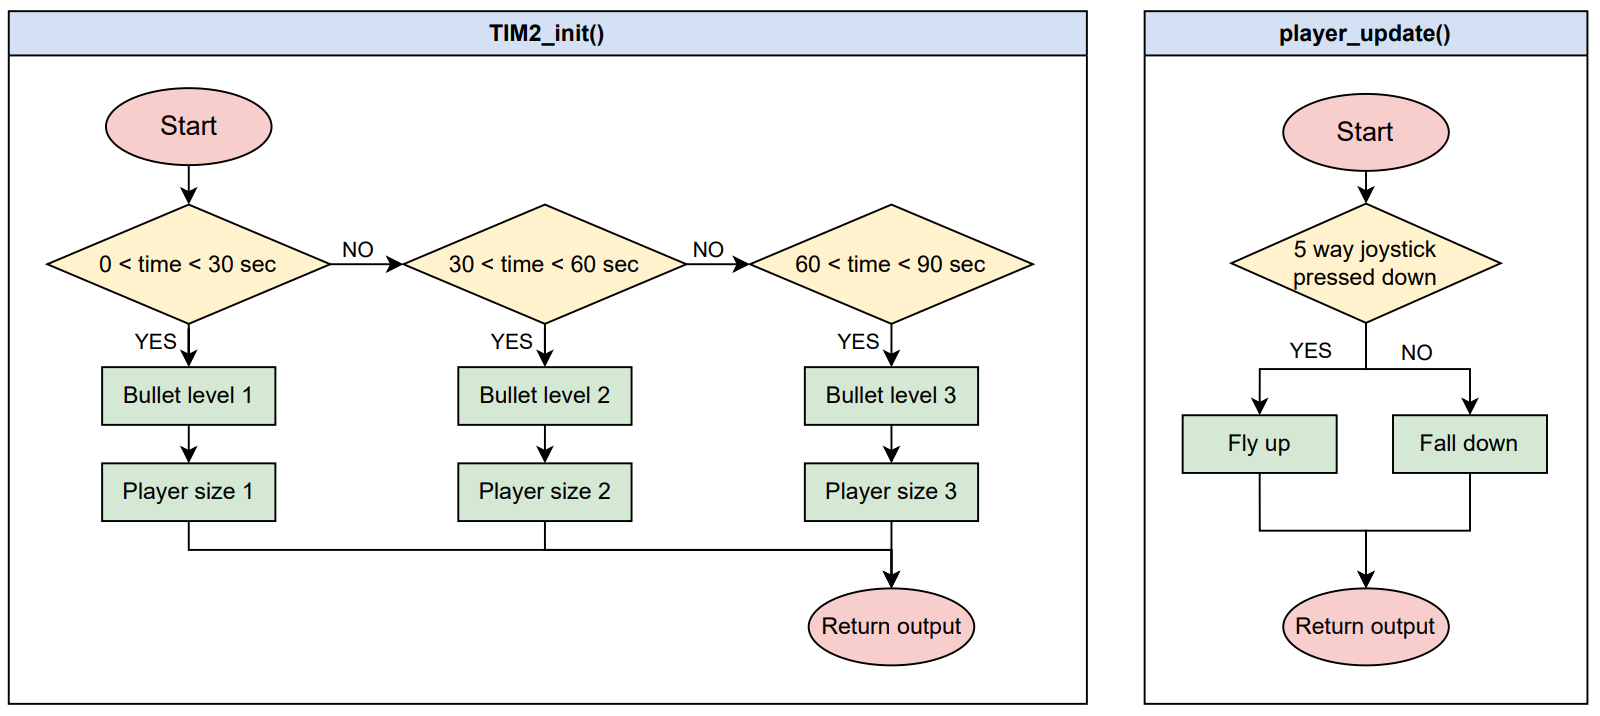
\includegraphics[width=\textwidth]{Picturs/Diagrammer/FINAL_FR_TIM_PLAYER.png}
    \caption{Flow diagram af TIM2\_init() \& player\_update()}
    \label{fig:TIME_PLAYER}
\end{figure}
\vspace{-2.5em}

Som illustreret i \lstinline!player_update()! diagrammet i figur \ref{fig:TIME_PLAYER}, er spillerens position afhængig af det input joysticket modtager. Hvis joysticket holdes ned vil karakteren bevæge sig opad og ellers vil den falde ned, som følge af spillets bevægelseslogik. Denne mekanisme er med til at sikre at spilleren kontinuerligt skal interager for at opretholde en stabil position. 

Som tidligere sagt er sværhedsgraden tidsbaseret, det er lige ledes illustrerede i figur \ref{fig:TIME_PLAYER} med \lstinline!TIM2_init()!. Her bruges en timer til at opdele spillet i forskellige tidsintervaller. Hvor projektil niveauet gradvis stiger, samt størrelsen på spilleren, hvilket vil gøre det sværere at undgå projektilerne. 

\subsection{Bullet position \& liv update} \label{chap:ProduktUdvikling_sec:skud_og_liv}
\vspace{0.5em}

\begin{figure}[H]
    \centering
    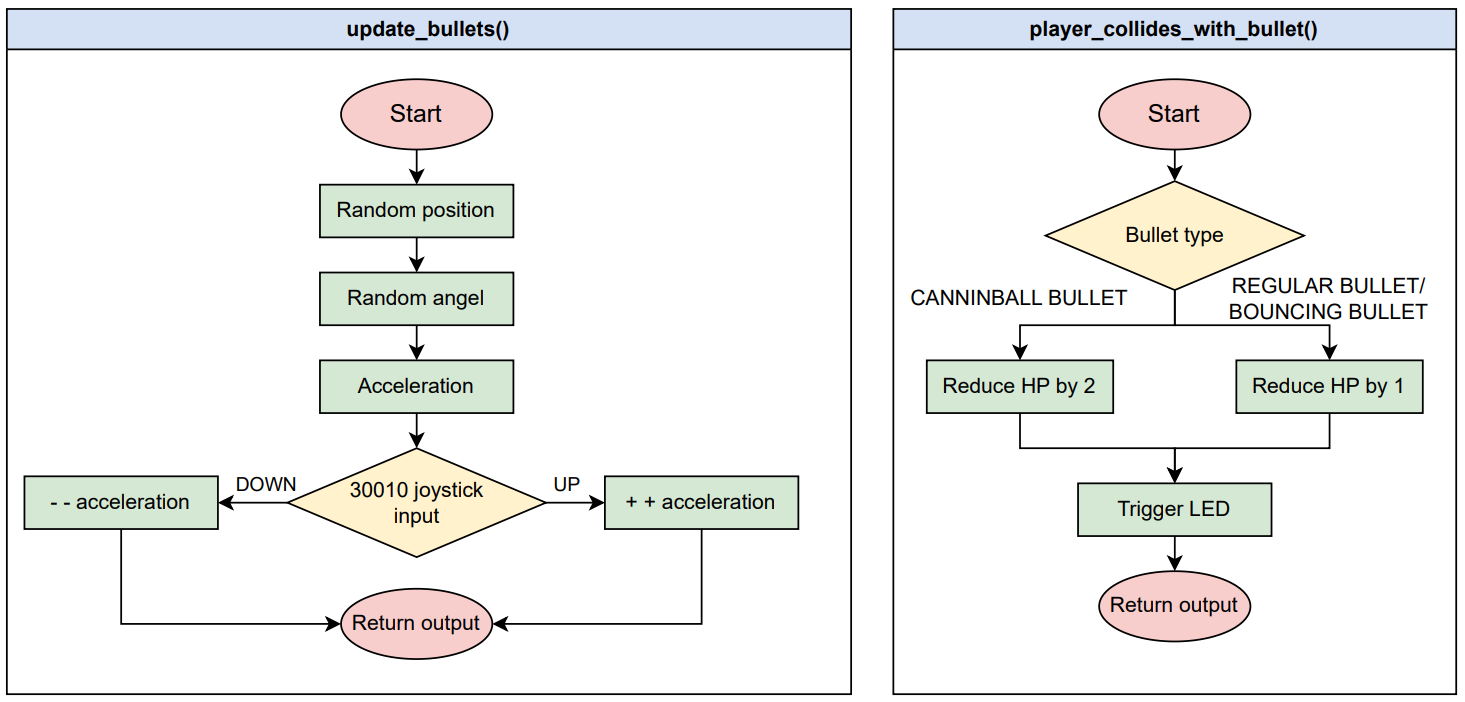
\includegraphics[width=\textwidth]{Picturs/Diagrammer/BULLRT_DIAGRAM.png}
    \caption{Flow diagram af update\_bullets() \& player\_collides\_with\_bullet()}
    \label{fig:bullet_live}
\end{figure}
\vspace{-2.5em}

For at håndtere projektiler og interaktionen med spillerne, benyttes funktionen \lstinline!update_bullets()! og \lstinline!player_collides_with_bullet()!. Som det fremgår i figur \ref{chap:ProduktUdvikling_sec:skud_og_liv}, gennemløber programmet alle aktive projektiler i hvert frame. Her opdateres projektilets position baseret på dets gældende hastighed og acceleration. En serlig feature i vores spil er at projektilernes acceleration styres af hardwaren, vha. et 30010 joystick.
Her gang et projektil opdateres, tjekkes der for kollision med spilleren. hvis spillerens koordinater overlapper med et projektil, vil spilleren mindste liv afhængig ag hvilke bullet type de har ramt. Ved kollision, aktiveres LED'en på hardwaren og giver spilleren et øjeblikkelig feedback på skaden.

\vspace{0.5em}
\subsection{Power ups} \label{chap:ProduktUdvikling_sec:powerups}
\vspace{0.5em}

På samme må måde som \lstinline!player_collides_with_bullet()! opfang om spilleren kolliderer med bullets bliver det også taget stilling til om der er kontakt med "powerups". Systemet sørge automatisk for at der med jævne mellemrum dukker power ups op på skærmen. De bevæger sig fra højre mod venstre, og spilleren skal aktivt navigere hen mod dem for at opsamle dem. Der findes tre forskellige typer. Når spilleren opsamler en power up aktivere det en specifik effekt. Hvor "liv" giver et ekstra liv, er de to andre tidsbaseret. Det betyder at spilleren kun har fordelen i et kort tidsrum, før spilleren vender tilbage til normal tilstand. Gennemgangen af disse afsnit viser, hvordan spillet er bygget op af forskellige moduler, der hver især har et specifikt ansvar. Ved at kombinere spillerens bevægelser, projektilernes baner og de taktiske fordele fra power-ups, skabes et sammenhængende spilsystem.